\documentclass[a4paper]{article}
\usepackage{listings}
\usepackage{graphicx}
\usepackage[scale=.7]{geometry}
\usepackage{amsmath}
\usepackage{float}
\usepackage{acronym}
\usepackage{cite}
\usepackage{url}
\usepackage[usenames, pdftex]{color}

\acrodef{WSM}[WSM]{Weighted Scan Matching}
\acrodef{ICP}[ICP]{Iterated Closest Point}
\acrodef{RANSAC}[RANSAC]{RANdom SAmple Consensus}
\acrodef{PFH}[PFH]{Point Feature Histograms}
\acrodef{FPFH}[FPFH]{Fast Point Feature Histograms}
\acrodef{SLAM}[SLAM]{Simultaneous Localization and Mapping}
\acrodef{PCL}[PCL]{Point Cloud Library}
\acrodef{SAC-IA}[SAC-IA]{SAmple Consensus Initial Alignment}

\title{Registration Using a RGB-D Camera\\
{\large Project A.I. / Individual Project}}

\author{Carsten van Weelden \\ 0518824 \\ \texttt{cvanweelden@gmail.com} \and Thomas van den Berg \\ 5789346 \\ \texttt{thomas.g.vandenberg@gmail.com} \and
 \small{Supervisor:} \\ Arnoud Visser \\ University of Amsterdam\\
  The Netherlands}

\date{\today}




\begin{document}
\maketitle

\section{Introduction}

In this project we familiarized ourselves with methods for 3D registration of images captured with cheap RGB-D sensors such as the Kinect. A Kinect mounted on a moving robot could replace both its RGB camera and its range finder. Another application would be affordable 3D reconstructions of objects or indoor scenes. For these applications we need to \emph{register} consecutive frames to the same global coordinate space. In effect, we need to find the transformation that the camera made in between the captured frames. %The robot's odometry can sometimes be used to get an initial estimate of the transformation, but in a scenario where the RGB-D camera is hand-held this is not possible. For this reason we focused on the registration step only. 

%Assuming that there is enough overlap between each pair of consecutive point clouds, we find a good registration by finding an optimal way to fit the two clouds.

%We experiment with different registration methods, and report on their performance and whether it degrades under certain circumstances.

The combined RGB and depth data forms a \emph{point cloud}. A standard method or registering two overlapping point clouds is the \ac{ICP} algorithm presented in \cite{besl1992method}. In this paper we show that simply registering each consecutive pair of frames using \ac{ICP} is not sufficient for good overall registration because errors in pair-wise registration accumulate quickly. We focus on the effect of only registering a subset of captured frames. Because this increases the magnitude of the transformation between frames we show that in this case it is better to use feature-based method to provide an initial guess to the \ac{ICP} algorithm.

\section{Background}

\subsection{ICP-based registration}

A basic method used in almost every approach to 3D registration is \ac{ICP}\cite{besl1992method}. It is an expectation maximization method that iteratively minimizes the distance between each point and its closest neighbor. Though \ac{ICP} is currently used mostly as a refinement step for more advanced algorithms, \ac{ICP} can be used as the main registration procedure in scene reconstruction \cite{izadi2011kinectfusion,newcombe2011kinectfusion} and \ac{SLAM} \cite{nuchter20076d}.

%In \cite{segal2009generalized}, an extension to \ac{ICP} was introduced that takes into account the local characteristics of the matched points. This Generalized-ICP gives a higher weight to point correspondence errors if they are in a direction perpendicular to the estimated plane. It is mentioned in both \cite{rusinkiewicz2001efficient} and \cite{segal2009generalized} that using this extension prevents the application of a closed-form solution to the minimization step.

%\ac{WSM} removes a simplyfying assumption from \ac{ICP}, namely that ``the range scans of different poses sample the environment's boundary at \emph{exactly} the same points''~\cite{pfister2002weighted}. In range scans, it often occurs that the points are much further apart in some areas of the model, because of the angle of the local surface or the distance from the sensor. The point-to-point error in these areas could easily be much greater, this is what the authors take into account by introducing an error which they name the \emph{correspondence error}. They model the variance of this error based on the distances to the closest model points, \cite{slamet2008boosting} give a clear illustration in their Figure 1. 

%In a sense, Generalized-ICP and \ac{WSM} are similar in that they make an explicit model of the error that the minimization step aims to minimize, based on the local characteristics. This has some clear advantages in terms of accuracy, but the extra computational costs are significant.

\subsection{Feature-based registration}

An alternative to \ac{ICP} based registration is feature-based registration in which the transformation between frames is estimated from correspondences between feature points in 3D space using \ac{RANSAC}. In stead of matching each point in the cloud to it's closest neighbor, characteristic \emph{descriptors} are calculated for each cloud. Based on these descriptors, the feature points are matched to their counterparts in the other frame to get a number of \emph{correspondences}. Not all these correspondences may be correct though, so \ac{RANSAC} is often used to filter the outliers. 

The approach we use is described in \cite{rusu2009fast} and uses \ac{FPFH} as descriptors. These features are based on the geometric properties of a local neighborhood. \ac{RANSAC} is then used to find the best feature point correspondences from which a rigid transformation is computed.

%For each point, these features are based on the properties of points in its neighborhood. To elaborate, every pair of points within the neighborhood (Figure~\ref{fig:fpfh}) generates a number of features based on their angle with respect to the local normal. Because the number of neighbors can vary, a histogram is created. Initially, every single point is used to generate a descriptor. Then, to speed up the matching and make it more robust, only \emph{unique} feature points are selected, i.e. points whose descriptors are different from the mean descriptor. \ac{RANSAC} is then used to find the best feature point correspondences.  

%\begin{figure}[htbp]
%    \centering
%        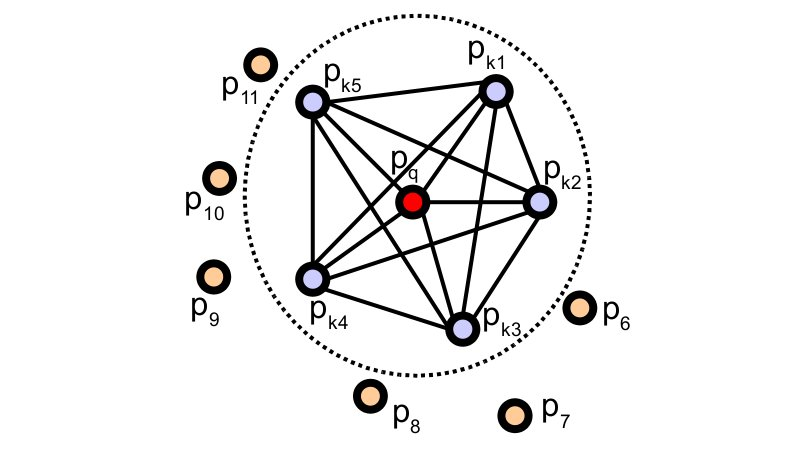
\includegraphics[height=4cm]{ims/fpfh.jpg}
%    \caption{The PFH dependency diagram (image from \cite{rusu2009fast}). It indicates that every pair of points in the neighborhood generates features.}
%    \label{fig:fpfh}
%\end{figure}

\subsection{Applications}

Global registration is the problem of reconstructing a global model from a sequence of frames. %Each frame has to be registered to a global coordinate system, generally defined by the axes of the first frame of the sequence. 
One challenge in applying registration algorithms to this problem is that errors in pairwise registration accumulate over time. In \cite{henry2010rgb} a method combining feature-based registration and \ac{ICP} is described. They use global consistency checking and loop closing to deal with registration noise and a surfel map to represent the global model.

%Other challenges associated with global registration are integrating the registered noisy measurements into a smooth global model.



%\subsection{\acf{SLAM}}

%This is also know as \emph{visual odometry} and a more complete overview can be found in \cite{scaramuzzavisual,fraundorfervisual}. 

By finding the relative transformation between frames we can also compute the egomotion of the camera\footnote{This problem is know as \emph{visual odometry} and a more complete overview can be found in \cite{scaramuzzavisual}.}, which can be used to perform \acf{SLAM}. In \cite{nuchter20076d} \ac{ICP} is used on point cloud data to solve the \ac{SLAM} problem in 3D. They use a cached version of the kd-tree data structure to make this feasible in real-time. They state that in combination with loop closing and model refinement this leads to accurate results.

%As mentioned before, the registration step that we focus on in this report provides us with all the information needed to perform \ac{SLAM} using \emph{visual odometry}. Visual odometry is the converse problem to registration: by finding the relative transformation between frames we can also compute the egomotion of the camera. A tutorial overview of visual odometry methods can be found in \cite{scaramuzzavisual,fraundorfervisual}. In \ac{SLAM} we use this registration step for localization, and by merging the registered 3D images we create a map of the environment. However, though the registration step is essential, it is far from sufficient for good localization. The most notable problem is the \emph{error buildup}; cumulative errors in the registration steps cause an ever greater error in the final position estimation. This can lead to a defective \emph{loop closing}: when the sensor comes to a place it has been before, the built-up error will almost surely cause this to be registered as a different position from the original one. If this loop can be detected at all, it is still necessary to re-register all earlier frames so that the loop is closed. 

%In \cite{pfingsthorn2008scalable} \ac{WSM} is combined with loop closing and a manifold data structure?


%%%%%%%%%%%%%%%%%%%%%%%%%%%%%%%%%%%%%%%%%%%%%%%%%%%%%%%%%%%%%%%%%%%%%%%%%%%%%%
%%%%%%                           EXPERIMENTS                            %%%%%%
%%%%%%%%%%%%%%%%%%%%%%%%%%%%%%%%%%%%%%%%%%%%%%%%%%%%%%%%%%%%%%%%%%%%%%%%%%%%%%


\section{Experiments}

We ran a number of experiments to find out about the behavior of different registration methods and their performance in different settings. One of the most influential properties of the input data is the magnitude of the transformation between frames. To clarify; a slow-driving robot will record frames that are are mostly similar, making it easier to find corresponding points or features in both frames, whereas a shaky handheld RGB-D camera might output frames with a much larger discrepancy. Typically, a set of frames with small transformations between them is an easier input to a registration algorithm. However, when building a global model or using the registration to perform SLAM, each step contributes an amount of error to the final results, therefore it is better to use as few frames as possible as long as the registration still works reasonably well.

Our first experiment examines how quickly the error increases as the distance between the input frames increases. These experiments consist of registering each frame $i$ to the $i-n^{\mathrm{th}}$ frame, with $n = {1,2,...,k}$. By skipping frames in this manner, we artificially create a larger transformation for the registration step to solve. 

The second experiment focuses on the trade-off between the error build-up from using a lot of frames and the increased error from skipping frames. We look at the error resulting from registering a pair of frames using different numbers of intermediate frames.

\subsection{Datasets}

We use two RGB-D datasets from the benchmark presented in \cite{sturm11rss-rgbd}. In addition to the RGB-D data, it contains a ground truth for the camera's position obtained using a motion capture system which we use for evaluation. Both datasets are captured as an indoor scene around a desk with several objects on it.

The specific datasets that we use are \texttt{freiburg2\_xyz} and \texttt{freiburg1\_desk}\footnote{Available at \url{http://cvpr.in.tum.de/data/datasets/rgbd-dataset}}. The \texttt{xyz} dataset was recorded with a slow and steady movement of the RGB-D sensor, so that the magnitude of the translation is constant. Rotation is kept to a minimum. The \texttt{desk} dataset is recorded with much faster movement, leading to larger differences between subsequent frames as well as motion blur and rolling shutter effects. It contains both translation and rotation between frames.

[[Only describe sofa set?]]
Additionally, we recorded two datasets ourselves using a Kinect sensor. The setup of this was as follows, we set up the Kinect on a wheeled cart to be able to create a stable and uniform motion. We then rode the cart around an object, trying to keep the camera pointing towards the object's center. We show qualitative results on the two datasets that we recorded ourselves.

\subsection{Implementation}

For our implementation we use \ac{PCL} \cite{Rusu_ICRA2011_PCL}. We use the standard \ac{ICP} implementation provided by this library with a maximum of 50 iterations. To set the maximum correspondence distance we tested values between 5cm and 25cm in 5cm increments on the first 200 frame pairs of the \texttt{desk} and took the value leading to the minimum rotation error, which was 15cm. We refer to this method in our figures as \texttt{ICP}.

 For our feature based method we use the implementation of the \ac{SAC-IA} method from \cite{rusu2009fast} as implemented for this library\footnote{This implementation does not apply the Levenberg-Marquardt algorithm as described in \cite{rusu2009fast}.}, limited to 1000 iterations with a maximum correspondence distance of 5cm and minimum distance of 0.5m between the samples used for the \ac{RANSAC} method. We optimized the feature radius  for the \ac{FPFH} features in the same manner as the \ac{ICP} parameter for values between 10 and 35cm, which lead to a minimum at 30cm. For the normal estimation radius we use a third of the feature radius. We refer to this method as \texttt{FPFH}. We also experiment with a combination of \ac{ICP} and \ac{FPFH} by using the output of the \ac{FPFH} registration as initial guess for the \ac{ICP} algorithm. We refer to this method as \texttt{FPFH+ICP} in our figures.
 
In all cases we remove sparse outliers by removing all points whose mean distance to its 50 nearest neighbors is more than one standard deviation from the overall mean and we subsample by taking one point for each 5cm$^3$ voxel.

%%%%%%%%%%%%%%%%%%%%%%%%%%%%%%%%%%%%%%%%%%%%%%%%%%%%%%%%%%%%%%%%%%%%%%%%%%%%%%
%%%%%%                           RESULTS                                %%%%%%
%%%%%%%%%%%%%%%%%%%%%%%%%%%%%%%%%%%%%%%%%%%%%%%%%%%%%%%%%%%%%%%%%%%%%%%%%%%%%%


\subsection{Frame-to-frame ICP results}

\begin{figure}[ht]
    \centering
        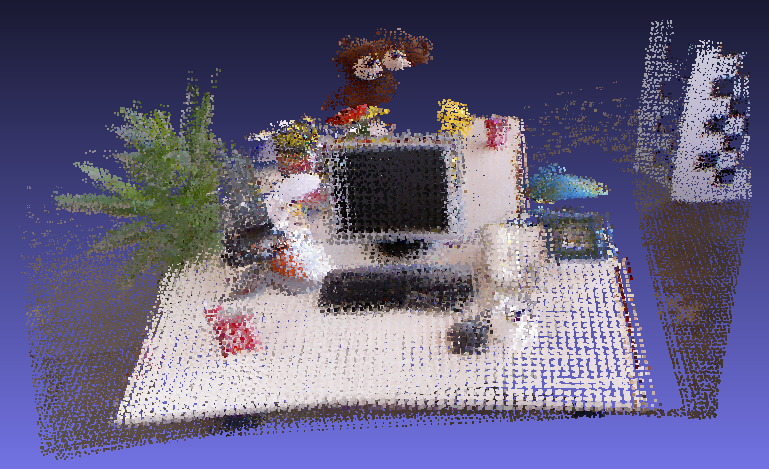
\includegraphics[width=\textwidth]{ims/xyz_results_f2f.png}
    \caption{Registration results on the \texttt{xyz} dataset using \ac{ICP} on each consecutive frame pair.}
    \label{fig:xyz_results_f2f}
\end{figure}

%Using \ac{FPFH} with \ac{ICP} we registered frames from the two datasets as well as from two datasets that we recorded ourselves. This section presents some of the qualitative results before we evaluate against the benchmark ground truth in the following sections.

We registered [[how many?]] frames from the \texttt{xyz} dataset using \ac{ICP} on each consecutive frame pair. The results are shown in Figure \ref{fig:xyz_results_f2f}. We see an obvious error in registration caused by inaccuracy in the frame-to-frame registration, as well as accumulated error over time as each registration step relies on the previous registrations. We investigate these sources of error in respectively Sections \ref{registration_error} and \ref{accumulated_error}.



%Figure \ref{fig:xyz_results} shows the result of registering the first [[how many?]] frames of the \texttt{xyz} dataset. We can clearly see the effect of errors in the pairwise registration where, after a single mis-estimation of the transformation between frames, all following frames are also badly registered, resulting in duplicate objects such as the teddy bear behind the desk and the calibration pattern to the right.




\subsection{Registration error}
\label{registration_error}

We show how the error for registering a frame pair increases as the frames are farther apart by computing the rotation and translation error for frame pairs with varying offsets between frames. Here we use the frame offset as a proxy for the magnitude of the transformation, but we also show how the rotation and translation magnitudes vary with the frame offset.

We calculate the rotation error as the angular distance between the true rotation $q$ and the estimated rotation $\hat q$ which we calculate as $min(\theta, 2\pi - \theta)$ where $\theta$ is the angle between the two rotations represented as quaternions: $\theta = 2 * cos^{-1}(q \cdot \hat q)$. %Dit hierboven heb ik opgeschreven omdat het nergens te vinden was.
The translation error is given as the Euclidean norm of the difference between the true and estimated translation. We compute the mean errors over 50 frame pairs for up to 2 seconds apart from the start of the \texttt{xyz} and \texttt{desk} datasets.

\subsubsection{Results}

Figures~\ref{fig:xyz_translation}, \ref{fig:desk_rotation}, and \ref{fig:desk_translation} show the rotation/translation error as the distance between registered frame pairs increases. The rotation error for the \texttt{xyz} dataset is not shown because this dataset contains no significant rotation of the camera. In each set of figures, the \emph{magnitude} of the estimated transformations is included, this is to give an intuition about the characteristics of the registration methods (e.g. we suspect that \ac{ICP} estimates transformations more conservatively compared to feature-based methods). 

\begin{figure}[H]
    \centering
        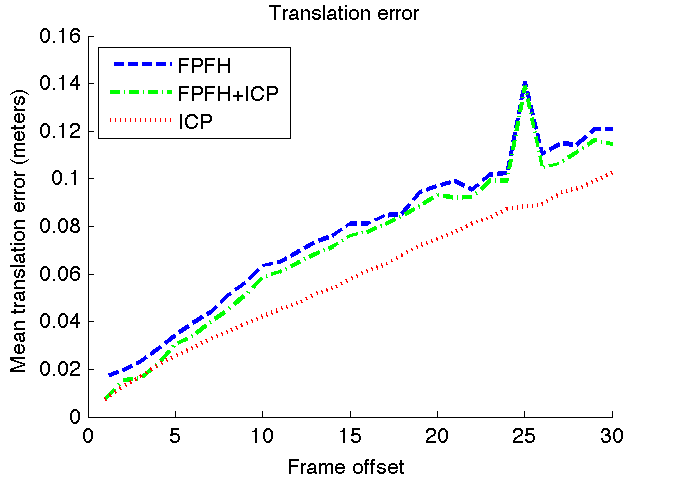
\includegraphics[width=0.49\textwidth]{ims/xyzTranslationerror.png}
        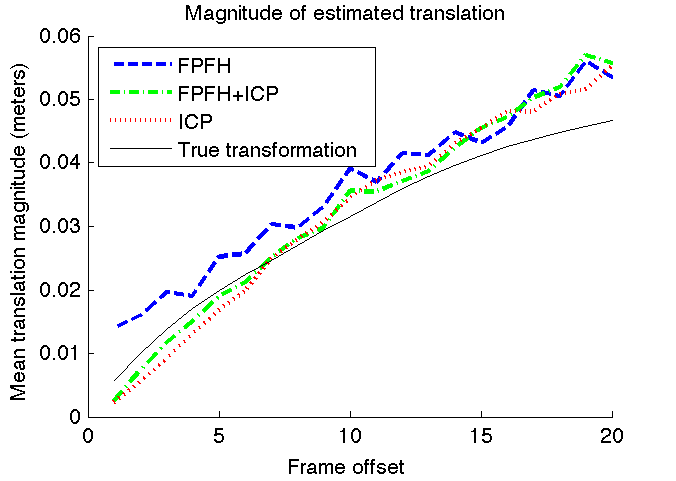
\includegraphics[width=0.49\textwidth]{ims/xyzMagnitudeofestimatedtranslation.png}
    \caption{\textbf{\texttt{xyz}}: The left image shows the translation error (i.e. the euclidian distance between the estimated translation and the ground truth translation), the right image shows \emph{magnitude} of the ground-truth translation and of those estimated.}
    \label{fig:xyz_translation}
\end{figure}

\begin{figure}[H]
    \centering
        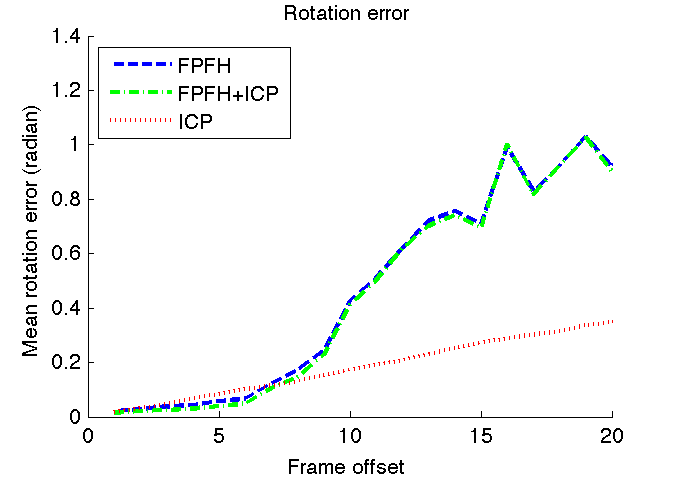
\includegraphics[width=0.49\textwidth]{ims/deskRotationerror.png}
        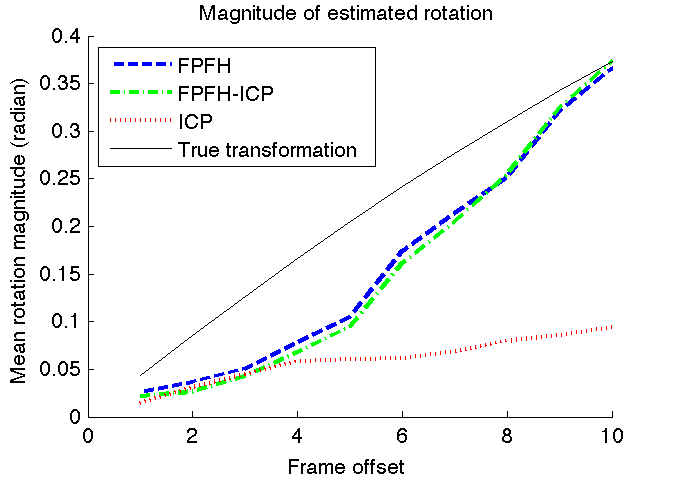
\includegraphics[width=0.49\textwidth]{ims/deskMagnitudeofestimatedrotation.png}
    \caption{\textbf{\texttt{desk}}: The left image shows the rotation error (i.e. the spherical distance between the estimated rotation and the ground truth rotation), the right image shows the \emph{magnitude} of the ground-truth rotation and of those estimated}
    \label{fig:desk_rotation}
\end{figure}

\begin{figure}[H]
    \centering
        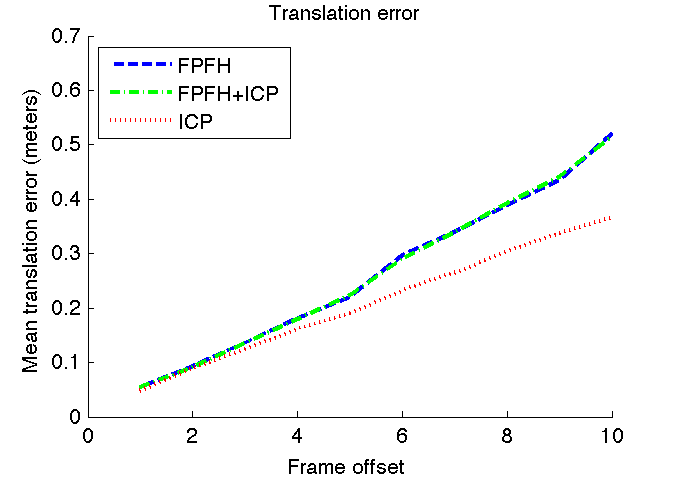
\includegraphics[width=0.49\textwidth]{ims/deskTranslationerror.png}
        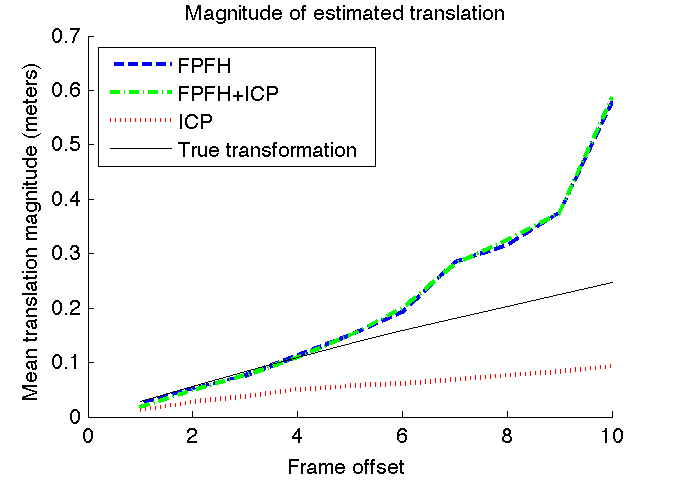
\includegraphics[width=0.49\textwidth]{ims/deskMagnitudeofestimatedtranslation.png}
    \caption{\textbf{\texttt{desk}}: The left image shows the translation error (i.e. the euclidian distance between the estimated translation and the ground truth translation), the right image shows \emph{magnitude} of the ground-truth translation and of those estimated.}
    \label{fig:desk_translation}
\end{figure}

Our intuition, namely that the combination of a feature-based initial alignment with an \ac{ICP} refinement can give the best results, is most clearly reflected in Figure~\ref{fig:desk_rotation}. However, when the discrepancy between frames gets larger (more frames are skipped), it seems like the \ac{FPFH} method starts failing. Even \ac{FPFH} combined with \ac{ICP} starts performing worse than pure \ac{ICP}. This is also visible in Figure~\ref{fig:desk_translation}. According these same figures \ac{ICP} underestimates the rotation and translation while the feature-based methods tend to come up with much larger transformations. The counterintuitive result is that the smaller transformations estimated by \ac{ICP} result in a smaller mean error, even though the ground truth transformation is larger. This effect might be because the feature-based method finds the \emph{wrong} feature correspondences when little overlap is available.

We thought that \ac{ICP} would only work with small transformations between frames, and that it's effectiveness would quickly decrease with increasing discrepancy between frames. This seemed to be the case when we did a qualitative analysis of the registration results by viewing the global models. However, this hypothesis does not seem to be confirmed by our experiments. The results displayed in the preceding figures seem to indicate that the error of pure \ac{ICP} increases less than that of the other methods. It is interesting to note that the same phenomenon seems to be present in Figure 3a in \cite{steinbruecker_sturm_cremers_iccv11}, though those results were obtained using G-ICP in stead of vanilla \ac{ICP}. The authors do not give an explanation as to \emph{why} G-ICP would be more robust against larger displacements. We think this might be caused by the fact that feature based methods are more likely to produce large transforms; making it likely that they produce large errors, whilst \ac{ICP} is more conservative.

\subsection{Error accumulation}
\label{accumulated_error}

The registration step registers a pair of frames with a certain error (which we investigate in section \ref{registration_error}. For global registration and \ac{SLAM} this error accumulates as frames are sequentially registered to previously registered frames. One way to deal with this problem is by skipping frames. Registering fewer frames means accumulating less error, but the overlap between each pair of frames needs to be large enough for successful registration. 

We investigate the effect of skipping frames by looking at the registration error after a fixed duration whilst using a varying number of intermediate frames. We calculate the mean error over 50 segments of 1 second starting at frame 1 to 50 for the \texttt{xyz} and \texttt{desk} datasets.

\subsubsection{Results}

Figure \ref{fig:accumulated_error} shows the translation/rotation error after registering frames over 1 second for the \texttt{desk} dataset. We see that increasing the number of frames skipped reduces the accumulated error for the feature-based methods up to a point where the error starts to increase over the base level for registering all frame pairs. Overlap between frames in this dataset is small because of the faster movement of the camera.  We don't show results on the \texttt{xyz} dataset here, results were similar but less pronounced because of the favorable conditions of that dataset. As expected, the optimal amount of frames used is different depending on the characteristics of the dataset.

\begin{figure}[htbp]
    \centering
        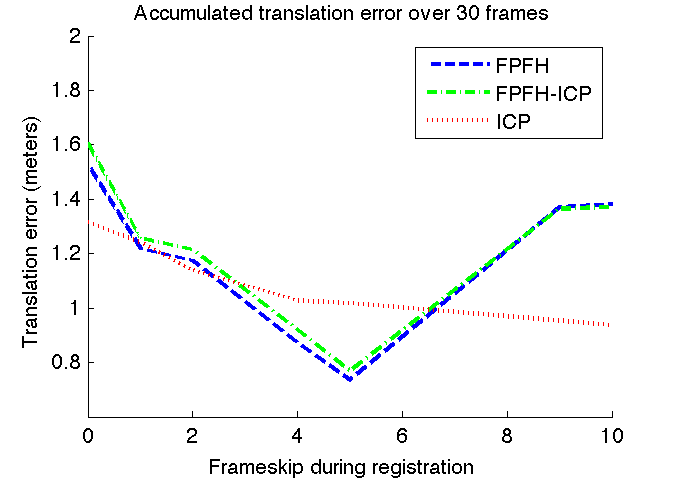
\includegraphics[width=0.49\textwidth]{ims/deskAccumulatedtranslationerrorover30frames.png}
        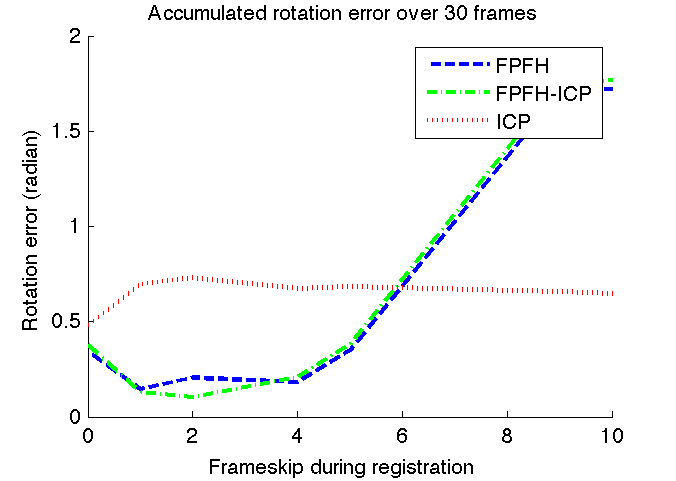
\includegraphics[width=0.49\textwidth]{ims/deskAccumulatedrotationerrorover30frames.png}
    \caption{Error built up after registering 30 consecutive frames (1 second) for the \texttt{desk} dataset.}
    \label{fig:accumulated_error}
\end{figure}

Figure~\ref{fig:accumulated_error} shows that there is an optimal selection of frames that yields the lowest error over longer periods. It shows that the feature-based methods have the least error buildup when skipping 4/5 frames between each pair. This reflects the tradeoff between limiting the amount of error accumulated over consecutive transformations and the error in the registrations themselves. Compared to \ac{ICP} the feature-based methods are better able to handle large transformations and thus have a more favorable balance between these two sources of error.

\subsection{Final results}

\begin{figure}[htbp]
    \centering
        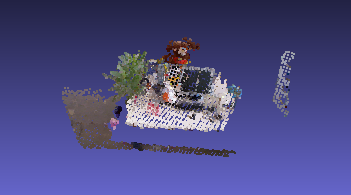
\includegraphics[width=\textwidth]{ims/xyz_results.png}
    \caption{Registration results on the \texttt{xyz} dataset using [[wat?]]}
    \label{fig:xyz_results}
\end{figure}

\begin{figure}[htbp]
    \centering
        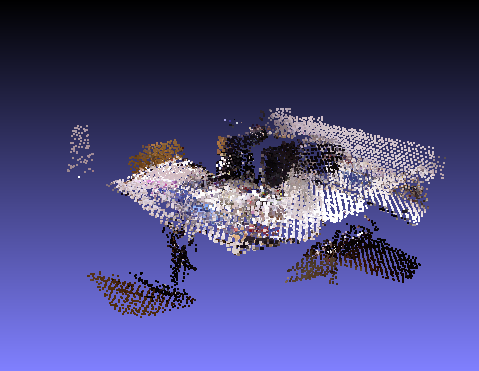
\includegraphics[width=\textwidth]{ims/desk_results.png}
    \caption{Registration results on the \texttt{desk} dataset using  [[wat?]]}
    \label{fig:desk_results}
\end{figure}

\begin{figure}[htbp]
    \centering
        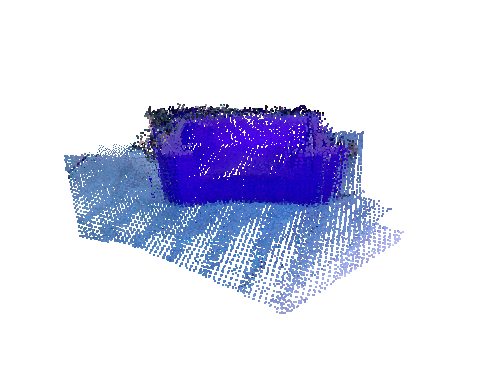
\includegraphics[width=\textwidth]{ims/sofa_results.png}
    \caption{Registration results on the \texttt{sofa} dataset using  [[wat?]]}
    \label{fig:sofa_results}
\end{figure}

%%%%%%%%%%%%%%%%%%%%%%%%%%%%%%%%%%%%%%%%%%%%%%%%%%%%%%%%%%%%%%%%%%%%%%%%%%%%%%
%%%%%%                           CONCLUSION                             %%%%%%
%%%%%%%%%%%%%%%%%%%%%%%%%%%%%%%%%%%%%%%%%%%%%%%%%%%%%%%%%%%%%%%%%%%%%%%%%%%%%%


\section{Conclusion}
Our first experiment showed that \ac{ICP} performs worse when few frames are skipped, but that its error increases constantly when skipping more frames, whereas a feature-based method performs better at first but degrades quickly at higher distances between frames. The question was then which of the methods would be more efficient when reducing error build-up by skipping as many frames as possible. Our second experiment shows that feature-based methods can outperform \ac{ICP} at optimal frame intervals, giving a minimal global error build-up.

\section{Discussion}
It is necessary to balance the performance of single pairs with the performance over a longer time. Using a fixed and constant portion of the frames (i.e. using every $n^{\mathrm{th}}$ frame) is generally a bad idea because most input data will not be homogeneous (i.e. the magnitude of the transformation between each pair of frames will vary). Therefore it is necessary to use a \emph{keyframe selection} method, which decides whether or not to discard each frame based on some initial estimation of it's utility. Depending on the application, there are a number of ways to drop poor frames. This depends on whether there is the opportunity to record viewpoints as desired, e.g. in situations where a robot has enough time to explore, or where the sensor is handheld and software runs real-time. If this is the case, one might simply perform the registration, \emph{verify} that the result is correct, and keep recording a certain viewpoint until enough coverage is obtained. \cite{makadia2006fully} mention such a method for verification in their Section 5. If there isn't an opportunity to actively revisit certain viewpoints, dropping bad frames can still be beneficial, but dropping too many frames might lead to gaps in the model, as the camera continues on its path.

\ac{ICP} only performs well when using very similar frames, but this will cause a large build-up of error. In all of the papers where \ac{ICP} was used without initial alignment, some extra techniques were used to prevent this, e.g. in \cite{izadi2011kinectfusion} a volumetric representation is used to create a global model, from which a reprojection is made to function as the model for \ac{ICP}. This global model is a compact representation that is less sensitive to the build-up of error.


%%%%%%
% PUT THIS WITH GLOBAL MODEL TEST
%%%%%%

%In \cite{slamet2008boosting} variants of \ac{ICP} are applied to solve the \ac{SLAM} problem in 2D, but instead of registering each frame to the previous frame they store all registered frames in a quad tree and register the frames against multiple previously registered frames. They show that this leads to better results than incremental pair-wise registration of frames.

%In the KinectFusion project presented in \cite{izadi2011kinectfusion,newcombe2011kinectfusion} \ac{ICP} is used to register depth frames captured using a Kinect camera to build a global model. They use a volumetric representation described in \cite{curless1996volumetric} to deal with registration noise and to provide a smooth model as result.
%Explain how this deals with registration noise and error build up.


\bibliography{../../literature/refs}{}
\bibliographystyle{apalike}

\end{document}
